\setchapterpreamble[u]{\margintoc}
\chapter{The Hydrogen Atom}
\labch{intro}

This is a very common and well study problem in quantum mechanics. The hydrogen atom is the simplest atom, and it is composed by a proton and an electron. The proton is located at the origin of the coordinate system, and the electron is located at a distance $r$ from the proton. The electron is described by a wave function $\psi(r,\theta,\phi)$, and the potential energy is given by the Coulomb potential. During this chapter we will go through all the theory and compare it with the result from the experiment done in the Modern Physics Lab.


\section{The electric potential}

The electric potential is well known since the 18th century. The potential is given by:

\begin{equation}
  \begin{array}{c}
    V(r) = -\frac{1}{4\pi\epsilon_0}\frac{Ze^2}{r}
  \end{array}
\end{equation}

Where $Z$ is the atomic number of the atom, $e$ is the absolut value of the charge of the electron, and $\epsilon_0$ is the vacuum permittivity. We are also going to define $\hbar$ as the Plank's constant and $m$ as the relative mass in this case, the mass of the electron. All these values are well known and the values get better every year. These values are:

\begin{equation}
  \begin{array}{c}
    e = 1.602176634 \cdot 10^{-19} \, \text{C} \\
    \epsilon_0 = 8.8541878128 \cdot 10^{-12} \, \frac{C^2 s^2}{kg m^2} \\
    m = 9.1093837015 \cdot 10^{-31} \, \text{kg}\\
    \hbar = 1.054571817 \cdot 10^{-34} \, \frac{kg m^2}{s}
  \end{array}
\end{equation}

We are going to look at the wave equation with natural units.

\begin{equation}
  \begin{array}{c}
    r = b u
    \\

    \\
    W_{E,j}(r=bu) = \chi_{E,j}(u)
  \end{array}
\end{equation}

So the wave equation is:

\begin{equation}
  \begin{array}{c}
  \frac{1}{b^2} \frac{d^2\chi}{du^2} + \frac{2(j+1)}{b^2 u}\frac{d \chi}{du} + \left(\frac{2mE}{\hbar^2} + \frac{2m}{\hbar^2}\frac{Ze^2}{4\pi\epsilon_0}\frac{1}{ub}\right)\chi = 0
  \\

  \\
  \frac{d^2\chi}{du^2} + \frac{2(j+1)}{u} \frac{d\chi}{du} + \left(\frac{2mEb^2}{\hbar^2}+\frac{2m}{\hbar^2}\frac{Ze^2 b}{4\pi\epsilon_0}\frac{1}{u}\right)\chi = 0
  \end{array}
\end{equation}

We want to find b so the term that belongs to the potential is equal to 1.

\begin{equation}
  \begin{array}{c}
    b = \frac{2\pi \epsilon_0 \hbar^2}{Z e^2 m} = [m] = \frac{1}{Z} 2.64588603 \cdot 10^{-19} m
  \end{array}
\end{equation}

That number is the natural atomic unit for length. The natural scal, b, becomes smaller with bigger Z.

We can also define the energy in natural units.

\begin{equation}
  \begin{array}{c}
    E = -\frac{\hbar^2}{2mb^2}\alpha
  \end{array}
\end{equation}

Where alpha can be either positive or negative. The wave equation looks like:

\begin{equation}
  \begin{array}{c}
    \frac{d^2\chi}{du^2} + \frac{2(j+1)}{u}\frac{d\chi}{du}-\alpha\chi +\frac{1}{u}\chi= 0
  \end{array}
\end{equation}

When u goes to infinite the equation become:

\begin{equation}
  \begin{array}{c}
    \frac{d^2\chi}{du^2} = \alpha\chi \rightarrow \chi = C_1 e^{-\sqrt{\alpha}u} - C_2 e^{\sqrt{\alpha}u}
  \end{array}
\end{equation}

Since $\chi$ has to go to 0 when $u$ goes to infinite, because of the normalization condition, $C_2$ is going to be 0 and alpha has to be postive, sowe can rewrite this in terms of:

\begin{equation}
  \begin{array}{c}
    \alpha=\beta^2
    \\

    \\
    E = -\frac{Z^2e^4m}{8\pi^2\epsilon_0^2\hbar^2}\beta^2
    \\

    \\
    \chi(u) = e^{-\beta u}R(u)
  \end{array}
\end{equation}

We are going to find the different terms in the wave equation separatly.

\begin{equation}
  \begin{array}{c}
    \frac{d^2\chi}{du^2} = \beta^2 e^{-\beta u} R - 2\beta e^{-\beta u} \frac{dR}{du}+e^{-\beta u} \frac{d^2R}{du^2}
    \\

    \\
    \frac{2(j+1)}{u} \frac{d\chi}{du} = \frac{-2(j+1)}{u} e^{\beta u} R + \frac{2(j+1)}{u} e^{\beta u} \frac{dR}{du}
    \\

    \\
    \left(\frac{1}{u}-\beta^2\right)\chi = \frac{1}{u} e^{\beta u}R -e^{\beta u} R
  \end{array}
\end{equation}

So the wave equation looks like:

\begin{equation}
  u\frac{d^2R}{du^2}+(2(j+1)-2\beta u)\frac{dR}{du} + (1 - 2(j+1)\beta)R = 0
\end{equation}

We can solve this differential equation using the power series method. We are going to assume that the solution is a power series.

\begin{equation}
  \begin{array}{c}
    R(u) = \sum_{k=0}^{\infty} C_k u^k
    \\

    \\
    \frac{dR}{du} = \sum_{k=0}^{\infty} C_{k+1} (k+1) u^{k}
    \\

    \\
    \frac{d^2R}{du^2} = \sum_{k=0}^{\infty} C_{k+1} k(k+1) u^{k-1}
  \end{array}
\end{equation}

We can substitute this into the wave equation, trying to match the indices of all the terms to the same $u^{k}$ and we get:

\begin{equation}
  \begin{array}{c}
    \sum_{k=0}^{\infty} C_{k+1} k (k+1) u^k +
    \\

    \\
    \sum_{k=0}^{\infty} C_{k+1} (k+1) 2(j+1) u^k -
    \\

    \\
    \sum_{k=0}^{\infty} C_{k} 2\beta k u^k +
    \\

    \\
    \sum_{k=0}^{\infty} C_{k} (1-2(j+1)\beta) u^k = 0
    \\

    \\
    \sum_{k=0}^{\infty} u^k\left[C_{k+1}\left[k(k+1)+2(k+1)(j+1)\right]+ \right.
    \\

    \\
    \left. C_k \left[ 1-2(j+1)\beta-2\beta k \right]\right] = 0
    \\

    \\
    C_k+1 =\frac{2\beta k-1+2\beta(j+1)}{(k+1)(k+2(j+1))}C_k = \frac{2\beta (k+j+1)}{(k+1)(k+2(j+1))} C_k
  \end{array}
\end{equation}

The power serie has to be finite because the $R_E,j(u)$ has to be normaliable. This means that for some k=p the coefficient $C_{p+1}$ has to be 0.

\begin{equation}
  \begin{array}{c}
    2\beta (p+j+1) -1 = 0
    \\

    \\
    \beta = \frac{1}{2(p+j+1)} = \frac{1}{2n}
  \end{array}
\end{equation}

Where n is $n=p+j+1$. Because p and j are define as integer numbers from 0 to infinte, n is an integer number, but from 1 to infinite. Now we can define the energy in terms of n.

\begin{equation}
  \begin{array}{c}
    E = -\frac{Z^2 e^4 m}{32\pi^2\epsilon_0^2\hbar^2 n^2}
  \end{array}
\end{equation}

That is the energy for the eigen-functions:

\begin{equation}
  \begin{array}{c}
    \psi_{n,j,m} = \left(\sum_{k=0}^{n-j-1} C_k u^k \right)e^{-\frac{1}{2n}u}(bu)P_j^m(\theta)e^{im\phi}
  \end{array}
\end{equation}

We can plot some of the eigen-functions to see how they look like.

\section{Eigen-functions of the hydrogen atom}


\begin{figure}
  \centering
  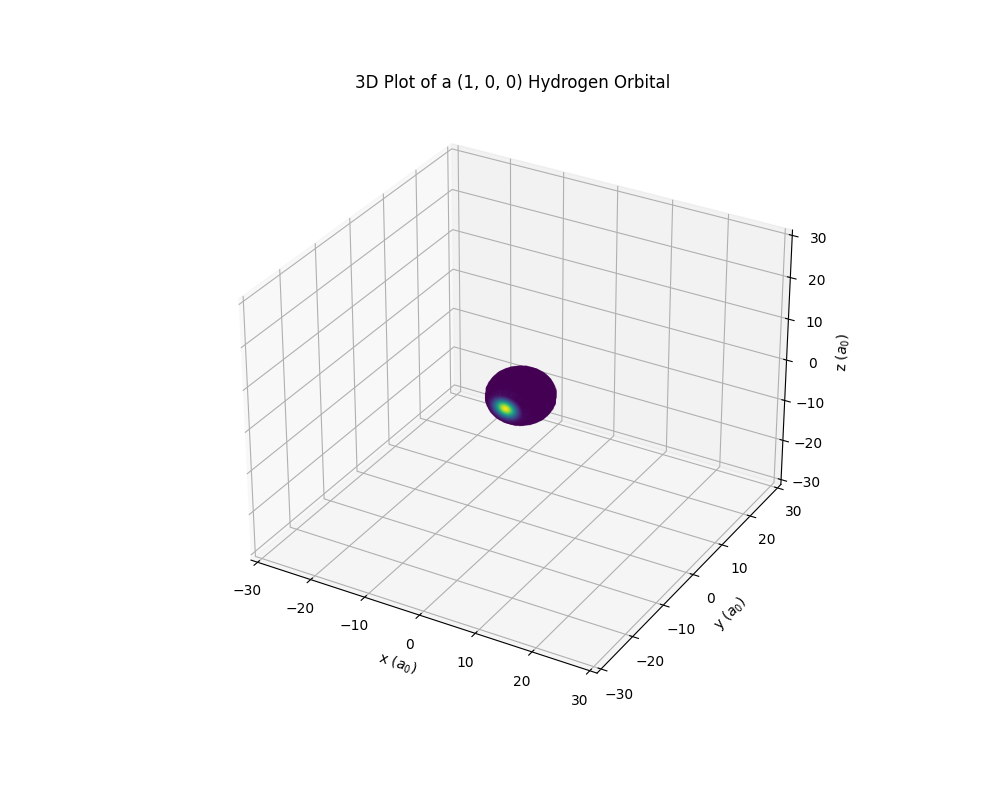
\includegraphics{images9/3d_plot_1,0,0.png}
  \caption{Probability distribution (n=1,j=0,m=0)}
\end{figure}

\begin{figure}
  \centering
  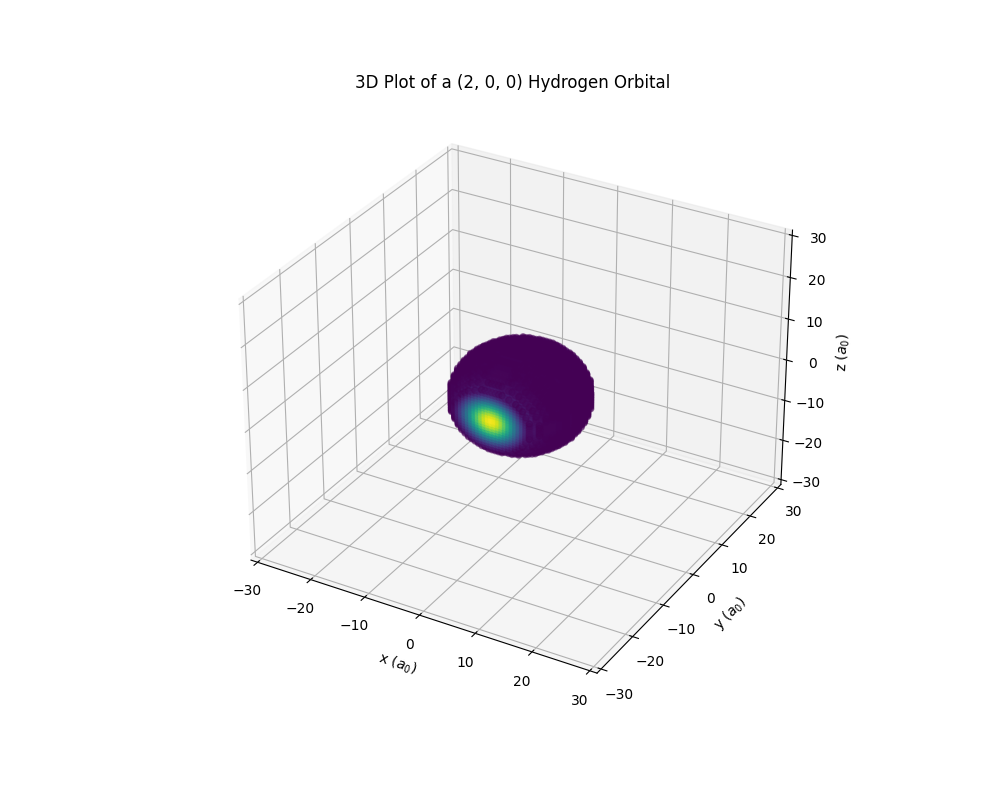
\includegraphics{images9/3d_plot_2,0,0.png}
  \caption{Probability distribution (n=2,j=0,m=0)}
\end{figure}

\begin{figure}
  \centering
  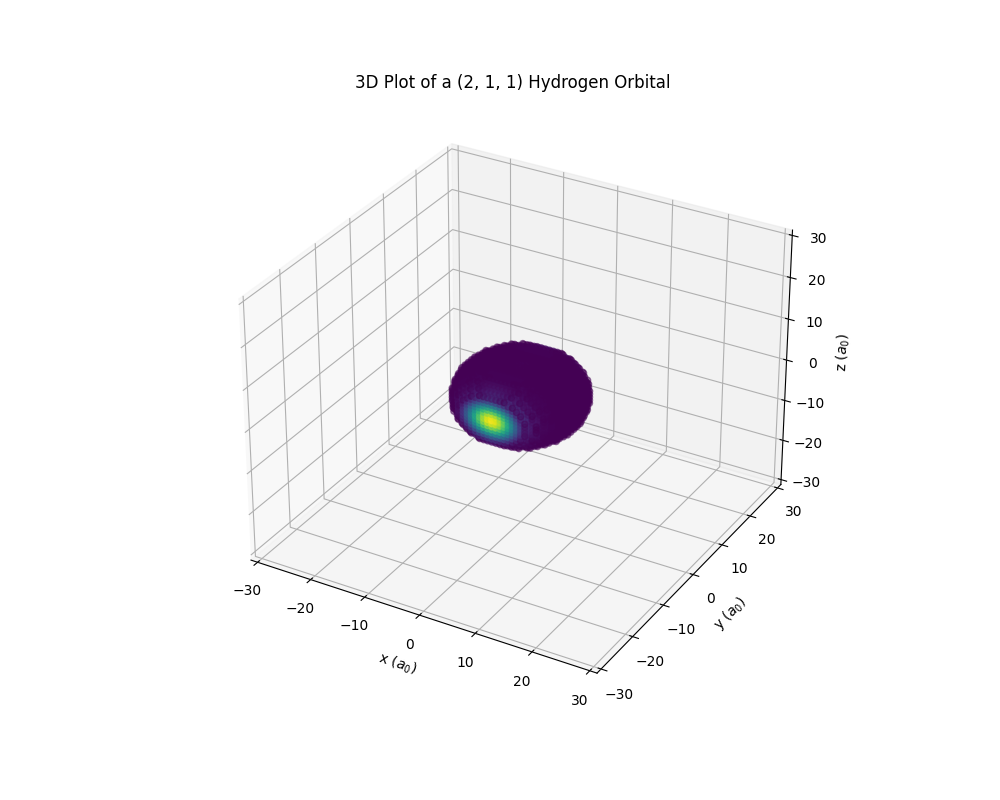
\includegraphics{images9/3d_plot_2,1,1.png}
  \caption{Probability distribution (n=2,j=1,m=1)}
\end{figure}

\begin{figure}
  \centering
  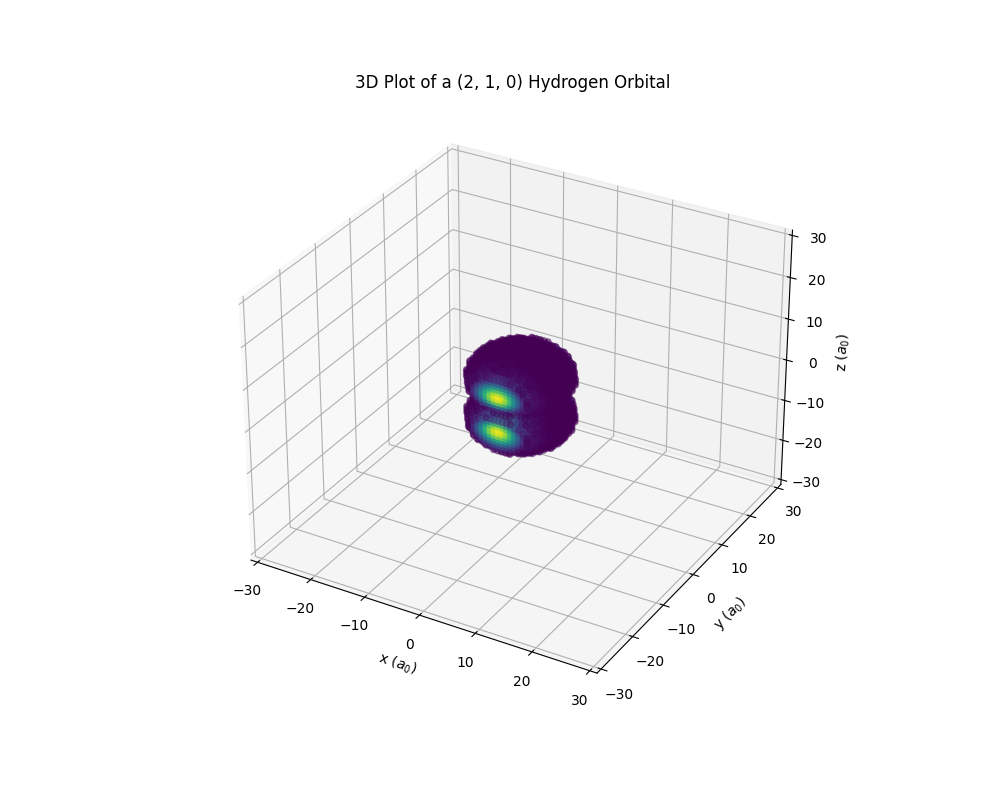
\includegraphics{images9/3d_plot_2,1,0.png}
  \caption{Probability distribution (n=2,j=1,m=0)}
\end{figure}

\begin{figure}
  \centering
  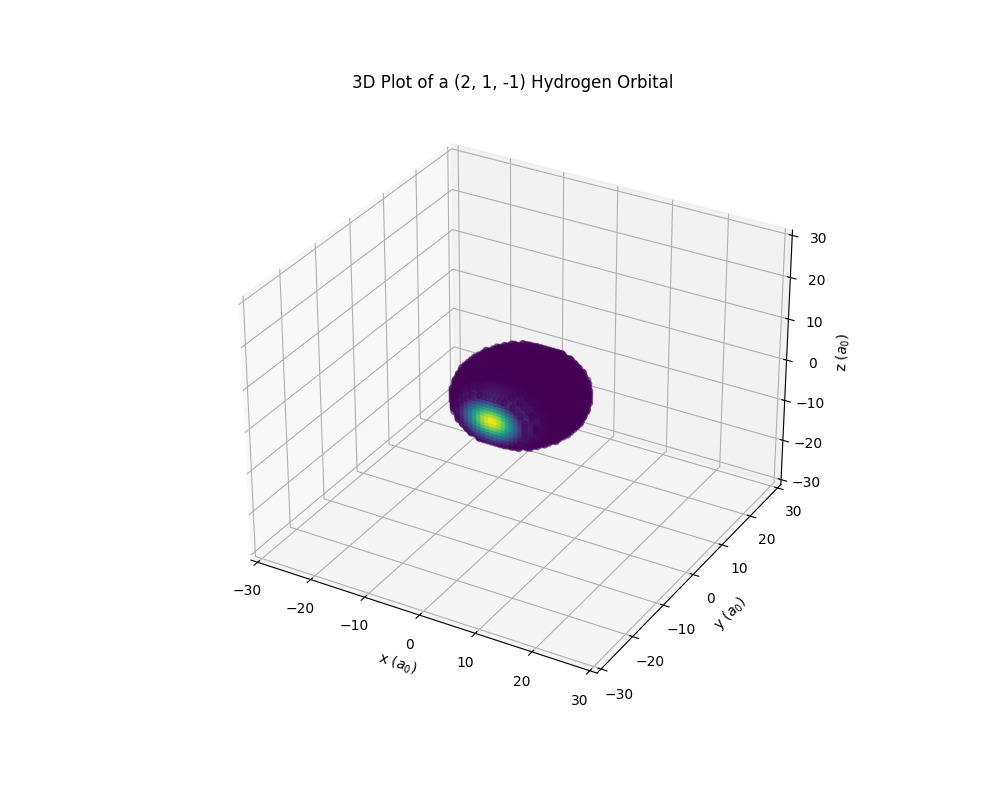
\includegraphics{images9/3d_plot_2,1,-1.png}
  \caption{Probability distribution (n=2,j=1,m=-1)}
\end{figure}


\section{Temperature and Light}

If we look at the plot of  the energy depending on n,we are going to see that the gap between the first energies is bigger than those of the higher energies. To move from one energy level to a higer one we need some temperature. The energy needed to move from the energy $E_i$ to $E_f$ is determined by the factor $KT$, where $K$ is the Boltzmann constant and $T$ is the temperature.

\begin{equation}
  \begin{array}{c}
    \Delta E = E_f - E_i = KT
  \end{array}
\end{equation}

This means that if the temperature is higher we will be able to reach higher energies. However the probability of the particle to be in the lowest energy is always greater or equal than the energy of the particle to be in a higher energy level. This is given by the Boltzmann distribution.

\begin{equation}
  \begin{array}{c}
    P(E_n) \propto e^{-\frac{E_n}{KT}}
  \end{array}
\end{equation}

In the same way we can see that energy can be emitted from the electron when it change from a higher energy to a lower energy state. This energy is going to be emitted in the form of light. The energy of the light is going to be the same as the energy difference between the two energy levels.

\begin{equation}
  \begin{array}{c}
    \Delta E = E_f - E_i = h\omega_{light}
  \end{array}
\end{equation}

